\section{Decomposition Rate with Respect to Dominant Fungi Traits}\label{sec:rate}

In this problem, the \textbf{hyphal extension rate} and \textbf{moisture tolerance} are the two basic dominating traits we need to consider in modeling the decay ability of the fungi community.

\begin{figure}\label{fig:rd-plot}
    \begin{minipage}{0.6\textwidth}
        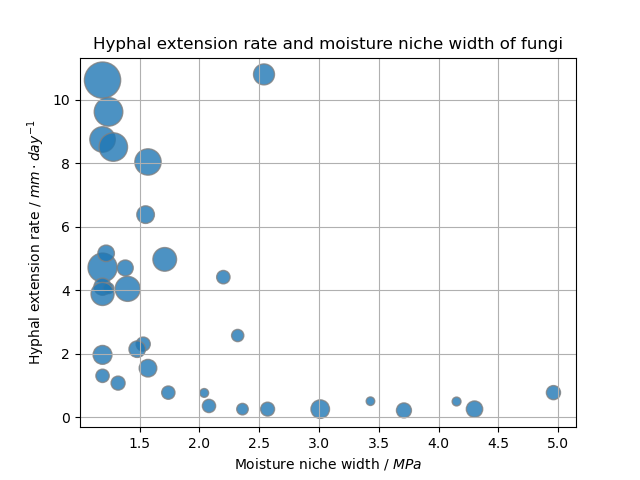
\includegraphics[width=\textwidth]{rd-plot.png}
    \end{minipage}
    \begin{minipage}{0.4\textwidth}
        \caption{Hyphal extension rate and moisture niche width of the fungi, size of the bubble represents he decomposition rate of logs after 122 days of decay}
    \end{minipage}
\end{figure}


\subsection{Decomposition rate model regarding hyphal extension rate, moisture tolerance and competitive ranking}


\begin{figure}
    \centering
    \begin{minipage}[t]{0.48\textwidth}
        \centering
        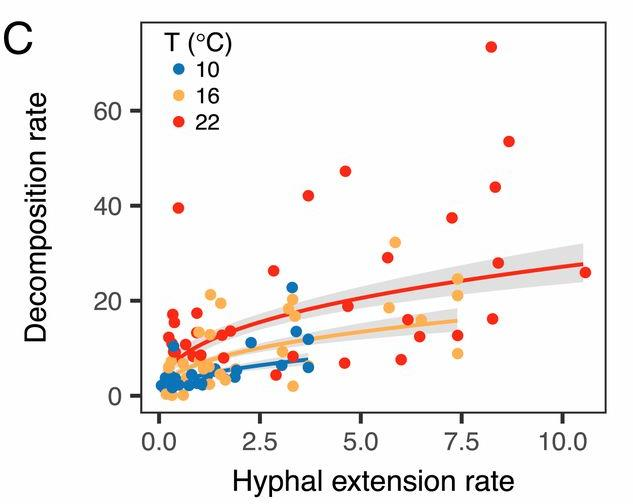
\includegraphics[width=0.8\textwidth]{figure1.jpg}
        \caption{The relationship between the hyphal extension rate (mm/day) of various fungi and the resulting wood decomposition rate (\% mass loss over 122 days) at various temperatures. This figure is adopted from \cite{Lustenshouwer}.}\label{fig:hyphal}
    \end{minipage}
    \begin{minipage}[t]{0.48\textwidth}
        \centering
        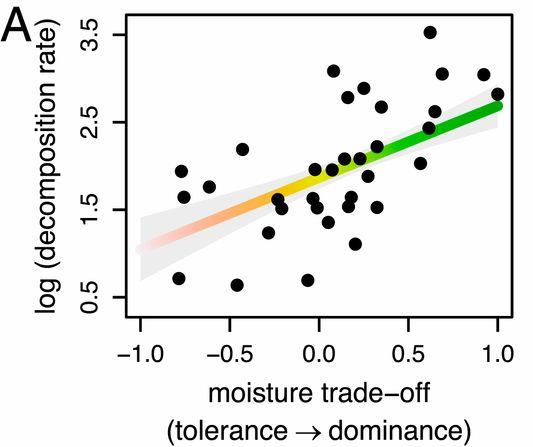
\includegraphics[width=0.8\textwidth]{figure2.jpg}
        \caption{The relationship between the moisture tolerance (difference of each isolate’s competitive ranking and their moisture niche width, both scaled to $[0,1]$) of various fungi and the resulting wood decomposition rate (\% mass loss over 122 days, log transformed). This figure is adopted from \cite{Lustenshouwer}.}\label{fig:moisture}
    \end{minipage}
\end{figure}


From Figure \ref{fig:hyphal} and Figure \ref{fig:moisture}, it is observed that the relation between the decomposition rate and hyphal extension rate, as well as between the log transformed decomposition rate and relative moisture tolerance are approximately linear.

\begin{equation}\label{eq:decay-ability}
    \left\{\begin{aligned}
         & D = k_1r + b_1     \\
         & \ln D = k_2m + b_2
    \end{aligned}\right.
\end{equation}

% Apparently, if the hyphal extension rate is $0$, the composition rate would also be $0$, hence the parameter $b_1$ is intrinsically $0$. The model is further specified as

% \begin{equation}\label{eq:decay-ability}
%     \left\{\begin{aligned}            &
%                           D = k_1r \\ &
%                           \ln D = k_2m + b_2.
%     \end{aligned}\right.
% \end{equation}

Note that, in \ref{fig:moisture}, the $x$-axis variable is not exactly the moisture tolerance (moisture niche width), instead is the difference of each isolate’s competitive ranking and their moisture niche width, in range $[-1, 1]$. Hence in the model, competitive ranking $c$ is taken into consideration. According to \cite{Maynard-data}, the moisture niche width is normalized as

\begin{equation}
    \begin{aligned}
        \hat{d}_i =
        \frac{d_i - d_\text{min}}{d_\text{max}}.
    \end{aligned}
\end{equation}


\subsection{Decomposition rate data fitting for single fungus isolate}

Based on the traits data of various species of fungus provided in \cite{Maynard-data}, and the resulting experimental decomposition rate in \cite{Lustenshouwer}, the fitting result is shown in table \ref{tb:para-122d} and figure \ref{fig:decom-hyphal-122d} and \ref{fig:decom-m-122d}.

\begin{figure}
    \centering
    \begin{minipage}[t]{0.48\textwidth}
        \centering
        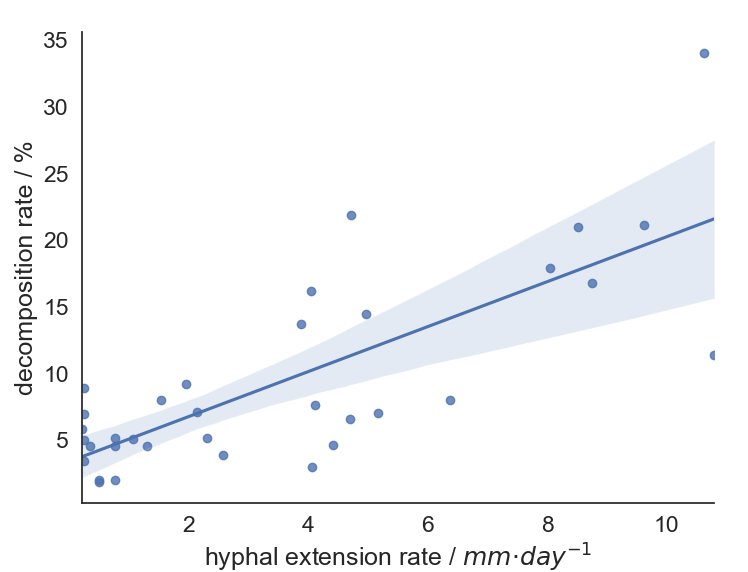
\includegraphics[width=\textwidth]{decom-hyphal-122d.png}
        \caption{The relationship between the hyphal extension rate of various fungi and the resulting wood decomposition rate. The hyphal extension rate is the geometrical average of the value tested under 10, 16 and 22 Celsius in \cite{Lustenshouwer}.}
        \label{fig:decom-hyphal-122d}
    \end{minipage}
    \begin{minipage}[t]{0.48\textwidth}
        \centering
        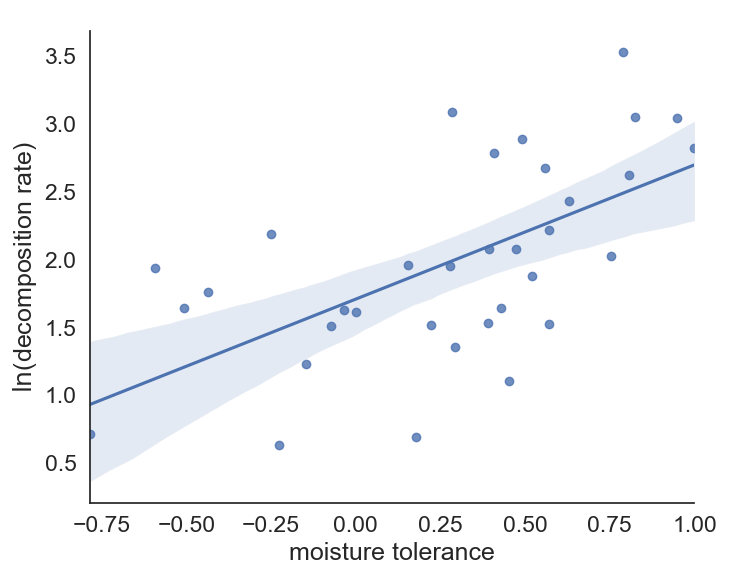
\includegraphics[width=\textwidth]{decom-m-122d.png}
        \caption{The  relationship  between  the  moisture tolerance. The tolerance-dominance trade-off is commonly found in the competition behavior of fungi. \cite{Maynard-data}}
        \label{fig:decom-m-122d}
    \end{minipage}
\end{figure}

\begin{table}
    \begin{minipage}{0.5\textwidth}
        \caption{The fitted parameters for the decay ability of an isolate over a short period}
        \label{tb:para-122d}
    \end{minipage}
    \begin{minipage}{0.5\textwidth}\centering
        \begin{tabular}{cccc}
            \toprule
            $k_1$  & $b_1$  & $k_2$  & $b_2$  \\
            \midrule
            1.6850 & 3.4082 & 0.5831 & 0.4896 \\
            \bottomrule
        \end{tabular}
    \end{minipage}
\end{table}


\subsection{Extending the model to multi-species system}

\begin{figure}
    \centering
    \begin{minipage}[t]{0.48\textwidth}
        \centering
        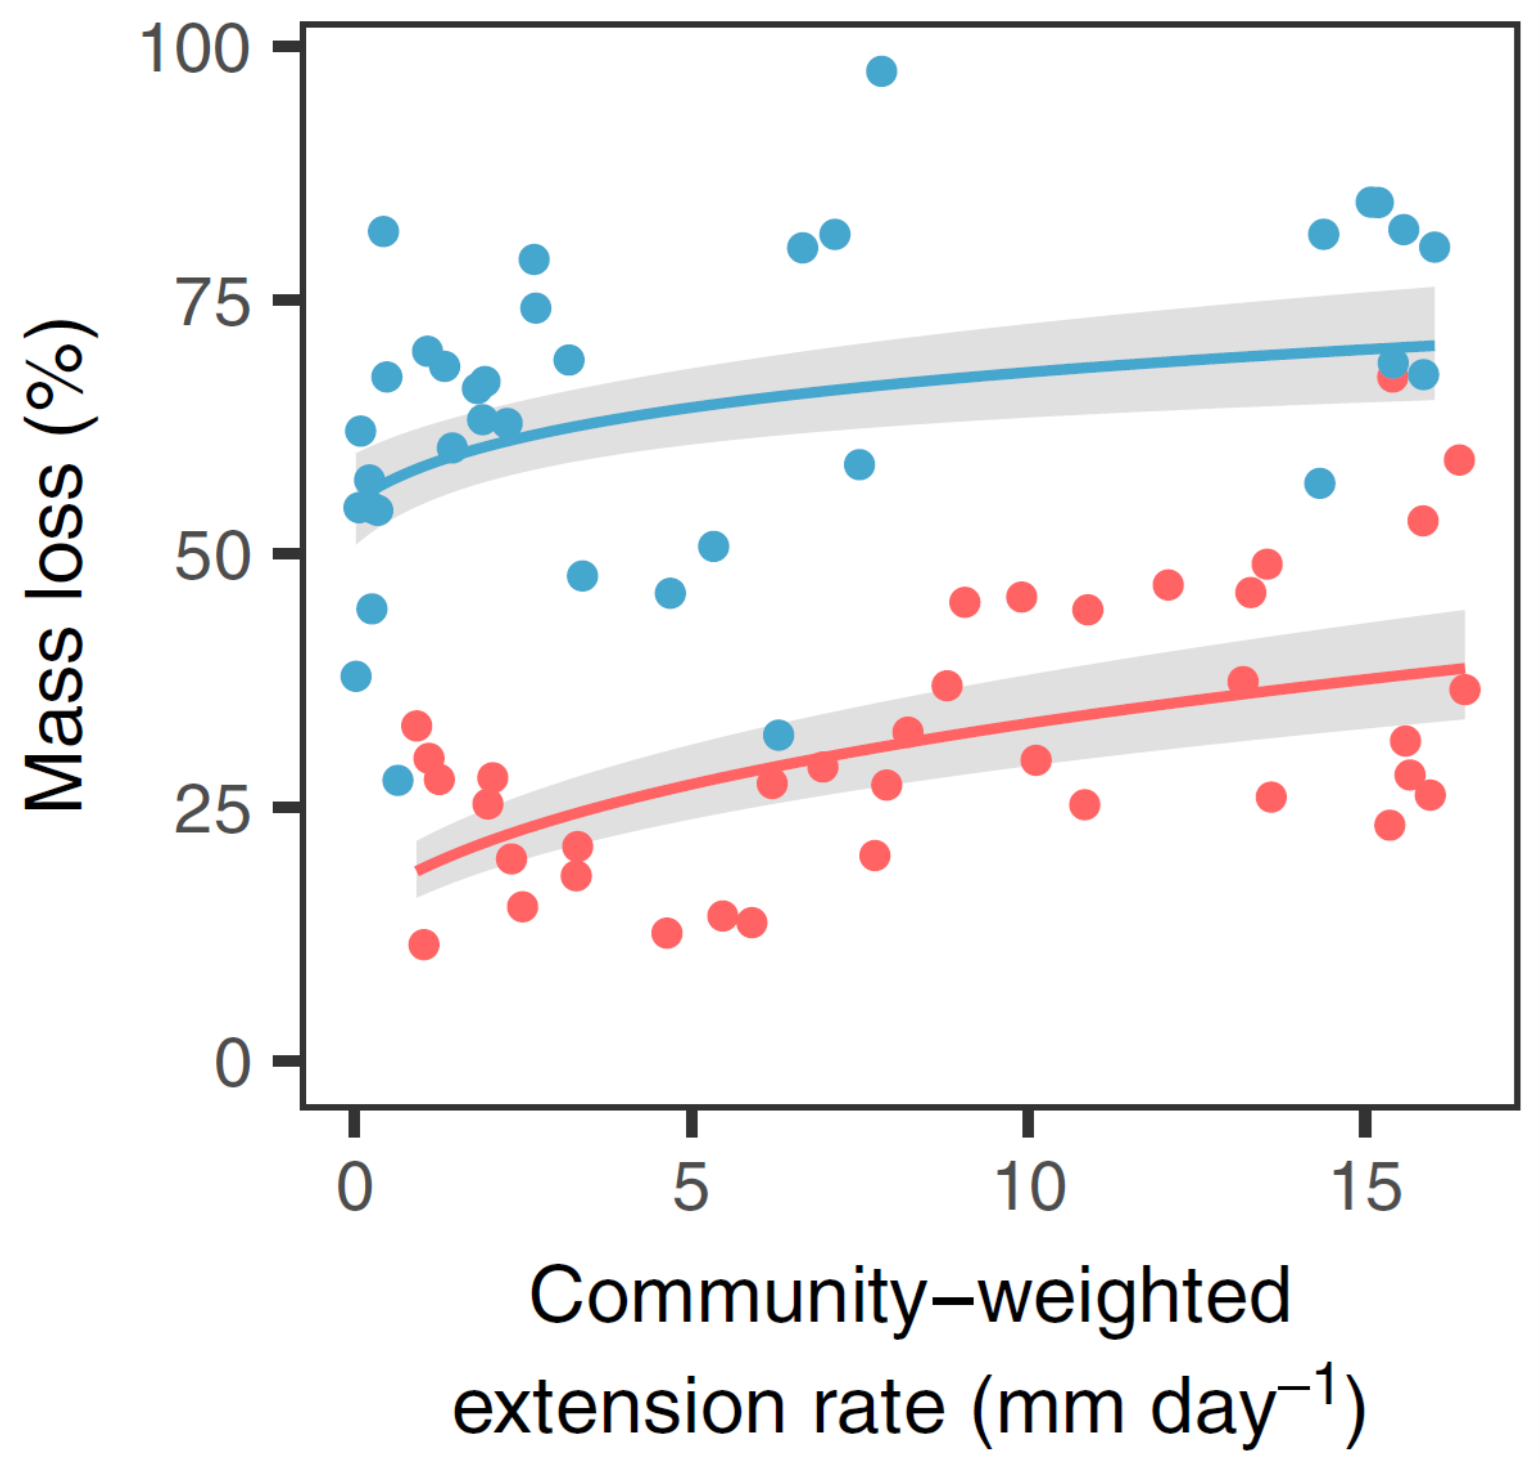
\includegraphics[width=0.8\textwidth]{figure3.png}
        \caption{The decomposition of logs increases with the hyphal extension rate of the fungal community that colonized them. This figure is adopted from \cite{Lustenshouwer}.}
        \label{fig:community}
    \end{minipage}
    \begin{minipage}[t]{0.48\textwidth}
        \centering
        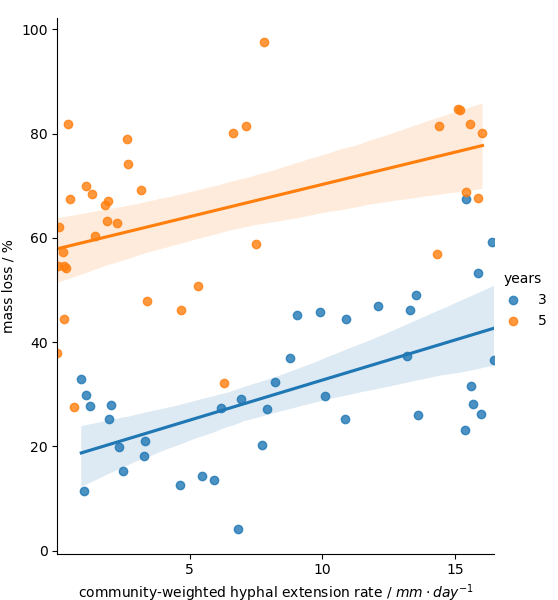
\includegraphics[width=\textwidth]{decom-year.png}
        \caption{The mass loss rate increases with the community-weighted hyphal extension rate. The experiments are conducted on a variety of wood substrates for 3 or 5 years.}
        \label{fig:decom-year}
    \end{minipage}
\end{figure}

For multi-species case, according to \ref{fig:community}, the decomposition of logs increases with the hyphal extension rate of the community, and is approximately characterized by a linear model with respect to the community-weighted mean extension rate. Therefore, in order to describe the decay ability of a community consists of multiple species of fungus, the relative quantity relation between of each isolate in the community is necessary.

The decay ability of a fungi community can be described quantitatively as the following expression.

\begin{equation}\label{eq:dcomm}
    D_\text{comm} =
    k_3\bar{r} + b_3=
    k_3\frac{r_1x_1 + \cdots + r_nx_n}{x_1 + \cdots + x_n} + b_3 =
    k_3\dfrac{\sum_{i=1}^n r_ix_i}{\sum_{i=1}^n x_i} + b_3.
\end{equation}

Research conducted in \cite{Lustenshouwer} presents the data obtained from experimental results on various wood substrate for 3 years or 5 years. With the data presented in \cite{Maynard-data}, the coefficient is roughly determined as in \ref{tb:para-year}, and the result is shown in figure \ref{fig:decom-year}.

\begin{table}
    \begin{minipage}{0.6\textwidth}
        \caption{The fitted parameters for the decay ability of a community over a long period}
        \label{tb:para-year}
    \end{minipage}
    \begin{minipage}{0.4\textwidth}\centering
        \centering
        \begin{tabular}{c|cc}
            \toprule
            Years & $k_3$ & $b_3$ \\
            \midrule
            3     & 1.539 & 17.32 \\
            5     & 1.237 & 57.87 \\
            \bottomrule
        \end{tabular}
    \end{minipage}
\end{table}

For solving this model for practical prediction of the decay ability of fungi community, each $x_i$ needs to be specified. This part is discussed in the following sections.
